\documentclass[12pt,final]{report}
\sloppy

\usepackage[utf8]{inputenc}

\title{Representing Ensembles of Molecules}
\author{Seth Denton Axen}
\date{August 2020}

\usepackage{graphicx}
\usepackage{caption}
\usepackage{subcaption}

% allow creating starred versions of commands
\usepackage{suffix}

% UCSF style
\usepackage[margin=1in]{geometry}
\usepackage{setspace} % Allows double spacing with the \doublespacing command
\usepackage{fancyhdr}
\renewcommand{\subsectionmark}[1]{\markboth{#1}{}}
\fancyhf{}
\renewcommand{\headrulewidth}{0pt}
\fancyfoot[C]{\thepage}
% not sure if this is necessary, but UCSF guidelines stress no widows or orphans
\usepackage[defaultlines=1,all]{nowidow}
\widowpenalty=100000
\clubpenalty=100000

% for adding title page and library release
\usepackage{pdfpages}

% use " as double quote
\usepackage[autostyle, english=american]{csquotes}
\MakeOuterQuote{"}

% E3FP paper preamble
\usepackage{siunitx}
\usepackage{amssymb}
\usepackage{upgreek}
\newcommand{\AUCsum}{AUC\textsubscript{SUM}}
\newcommand{\LEunit}{kcal/mol/heavy atom}
\newcommand{\axbx}[2]{\(\upalpha\)#1\(\upbeta\)#2}
\newcommand{\ax}[1]{\(\upalpha\)#1}
\newcommand{\Mx}[1]{M\textsubscript{#1}}
\newcommand{\ICfifty}{\(IC_\text{50}\)}
\newcommand{\Ki}{\(K_i\)}
\DeclareSIUnit{\molar}{M}
\sisetup{per-mode=symbol, detect-weight=true, detect-family=true}

% bibliography data
\usepackage[
  backend=biber,
  style=nature,
  natbib=true,
  sortlocale=en_US,
  url=false, 
  doi=true,
  eprint=false,
  backref=true,
  maxbibnames=99,
]{biblatex}
\addbibresource{references.bib}
\preto\fullcite{\AtNextCite{\defcounter{maxnames}{99}}}

% table formatting
\usepackage{tabularx}
\usepackage{booktabs}

% math
\usepackage{amsmath}
\raggedbottom{}

% really wide hat
% https://tex.stackexchange.com/questions/100574/really-wide-hat-symbol/101136
\usepackage{scalerel,stackengine}
\stackMath
\newcommand\reallywidehat[1]{%
\savestack{\tmpbox}{\stretchto{%
  \scaleto{%
    \scalerel*[\widthof{\ensuremath{#1}}]{\kern.1pt\mathchar"0362\kern.1pt}%
    {\rule{0ex}{\textheight}}%WIDTH-LIMITED CIRCUMFLEX
  }{\textheight}% 
}{2.4ex}}%
\stackon[-6.9pt]{#1}{\tmpbox}%
}
\parskip 1ex

% theorems
\usepackage{amsthm}
\usepackage{physics}
\usepackage{thmtools}
\newtheorem{theorem}{Theorem}[section]
\newtheorem{corollary}{Corollary}[theorem]
\newtheorem{lemma}[theorem]{Lemma}

%% symbols
\newcommand{\torus}{\mathbb{T}}
\newcommand{\mset}[1]{\mathcal{#1}}
\newcommand{\manifold}[1]{\mset{#1}}
\newcommand{\group}[1]{\mset{#1}}
\newcommand{\liealg}[1]{\mathfrak{#1}}
\newcommand{\dual}[1]{\hat{#1}}
%%% basic types
\renewcommand{\vec}[1]{\MakeLowercase{#1}}
\newcommand{\mat}[1]{\MakeUppercase{#1}}
%%% operations
\newcommand{\conj}[1]{{#1}^*}
\newcommand{\trans}[1]{{#1}^\mathrm{T}}
\newcommand{\invtrans}[1]{{#1}^{-\mathrm{T}}}
\newcommand{\hconj}[1]{{#1}^\mathrm{H}}
\newcommand{\invhconj}[1]{{#1}^{-\mathrm{H}}}
\newcommand{\sign}{\operatorname{sign}}
\newcommand{\diag}{\operatorname{diag}}
\newcommand{\expm}{\operatorname{Exp}}
\newcommand{\logm}{\operatorname{Log}}
\newcommand{\convwith}{*}
\newcommand{\expect}[2]{\left\langle #1 \right\rangle_{#2}}
\newcommand{\coef}[1]{\hat{#1}}
\newcommand\ftrans[1]{\mathcal{F}\qty[#1]}
\WithSuffix\newcommand\ftrans*[1]{\mathcal{F}[#1]}
\newcommand\finvtrans[1]{\mathcal{F}^{-1}\qty[#1]}
\WithSuffix\newcommand\finvtrans*[1]{\mathcal{F}^{-1}[#1]}
\newcommand{\finversion}[1]{{#1}^{\dagger}}
\newcommand{\inner}[2]{\left\langle #1, #2 \right\rangle}
%%% differential types
\newcommand{\Dtan}[1]{\dot{#1}} % tangent
\newcommand{\Dcot}[1]{\overline{#1}} % cotangent
%%% shorthand for specific objects
\newcommand{\bbR}{\mathbb{R}}
\newcommand{\bbC}{\mathbb{C}}
\newcommand{\SE}[1]{\group{SE} (#1)}
\newcommand{\se}[1]{\liealg{se} (#1)}
\newcommand{\SO}[1]{\group{SO} (#1)}
\newcommand{\so}[1]{\liealg{so} (#1)}
\newcommand{\Transg}[1]{\group{T} (#1)}
\newcommand{\transg}[1]{\liealg{t} (#1)}
\newcommand{\SU}[1]{\group{SU} (#1)}
\newcommand{\su}[1]{\liealg{su} (#1)}
\newcommand{\GL}[1]{\group{GL} (#1)}
\newcommand{\gl}[1]{\liealg{gl} (#1)}
\newcommand{\GA}[1]{\group{GA} (#1)}
\newcommand{\ga}[1]{\liealg{ga} (#1)}
\newcommand{\im}{i}
\newcommand{\bodyframe}[1]{\mathcal{#1}}
\newcommand{\diffnorm}{\operatorname{DiffNormal}}
\newcommand{\ie}{\emph{i.e.},~}
\newcommand{\eg}{\emph{e.g.},~}

% code formatting
\usepackage{sourcecodepro} % support more UTF-8 characters
\usepackage{minted} % syntax highlighting
\newminted{julia}{frame=lines,framesep=2mm}

% PGFPlotsX.jl preamble built by Plots.jl
\usepackage{pgfplots}
\pgfplotsset{compat=newest}
\usepgfplotslibrary{groupplots}
\usepgfplotslibrary{polar}
\usepgfplotslibrary{smithchart}
\usepgfplotslibrary{statistics}
\usepgfplotslibrary{dateplot}
\usetikzlibrary{arrows.meta}
\usetikzlibrary{backgrounds}
\usepgfplotslibrary{patchplots}
\usepgfplotslibrary{fillbetween}
\pgfplotsset{%
layers/standard/.define layer set={%
    background,axis background,axis grid,axis ticks,axis lines,axis tick labels,pre main,main,axis descriptions,axis foreground%
}{grid style= {/pgfplots/on layer=axis grid},%
    tick style= {/pgfplots/on layer=axis ticks},%
    axis line style= {/pgfplots/on layer=axis lines},%
    label style= {/pgfplots/on layer=axis descriptions},%
    legend style= {/pgfplots/on layer=axis descriptions},%
    title style= {/pgfplots/on layer=axis descriptions},%
    colorbar style= {/pgfplots/on layer=axis descriptions},%
    ticklabel style= {/pgfplots/on layer=axis tick labels},%
    axis background@ style={/pgfplots/on layer=axis background},%
    3d box foreground style={/pgfplots/on layer=axis foreground},%
    },
}
\usepackage{tikzscale}
% cache generated pdf files for faster compilation of LaTeX documents
\usepgfplotslibrary{external}
\tikzexternalize

% reference formatting
\usepackage{hyperref}
\usepackage{nameref}
\usepackage{chngcntr}
\usepackage{doi}
\counterwithin{figure}{chapter}
\counterwithin{table}{chapter}
\counterwithin{equation}{chapter}
\usepackage[capitalize, nameinlink]{cleveref}
\crefdefaultlabelformat{#2#1#3}
\creflabelformat{figure}{#2\textbf{#1}#3}
\crefname{figure}{\textbf{Fig.}}{\textbf{Figs.}}
\Crefname{figure}{\textbf{Fig.}}{\textbf{Figs.}}
\creflabelformat{table}{#2\textbf{#1}#3}
\crefname{table}{\textbf{Table}}{\textbf{Tables}}
\Crefname{table}{\textbf{Table}}{\textbf{Tables}}
\crefname{equation}{Eq.}{Eqs.}
\Crefname{equation}{Eq.}{Eqs.}
\crefname{theorem}{Theorem}{Theorems}
\Crefname{theorem}{Theorem}{Theorems}
\crefname{corollary}{Corollary}{Corollaries}
\Crefname{corollary}{Corollary}{Corollaries}
\crefname{lemma}{Lemma}{Lemmas}
\Crefname{lemma}{Lemma}{Lemmas}

% \usepackage[acronym,xindy]{glossaries}
% \makeglossaries
% \loadglsentries{glossary}

% commas between consecutive footnote superscripts
\usepackage{fnpct}

% for todo entries
\usepackage[colorinlistoftodos]{todonotes}
\makeatletter % single spacing in to-do notes
\renewcommand{\todo}[2][]{%
    \tikzexternaldisable % don't hide with tikzexternalize
    \@todo[caption={#2}, #1,inline]{\begin{spacing}{0.75}#2\end{spacing}}%
    \tikzexternalenable
} 
\makeatother
\newcommand{\insertref}[1]{\todo[color=green!40]{#1}}

% for line numbers
% \usepackage{lineno}
% \linenumbers

\usepackage{subfiles} % enable per-chapter compilation

\begin{document}

% FRONTMATTER

\pagestyle{plain} % no headers

% UCSF as of Summer 2020 does not include the title page
\pagenumbering{roman}

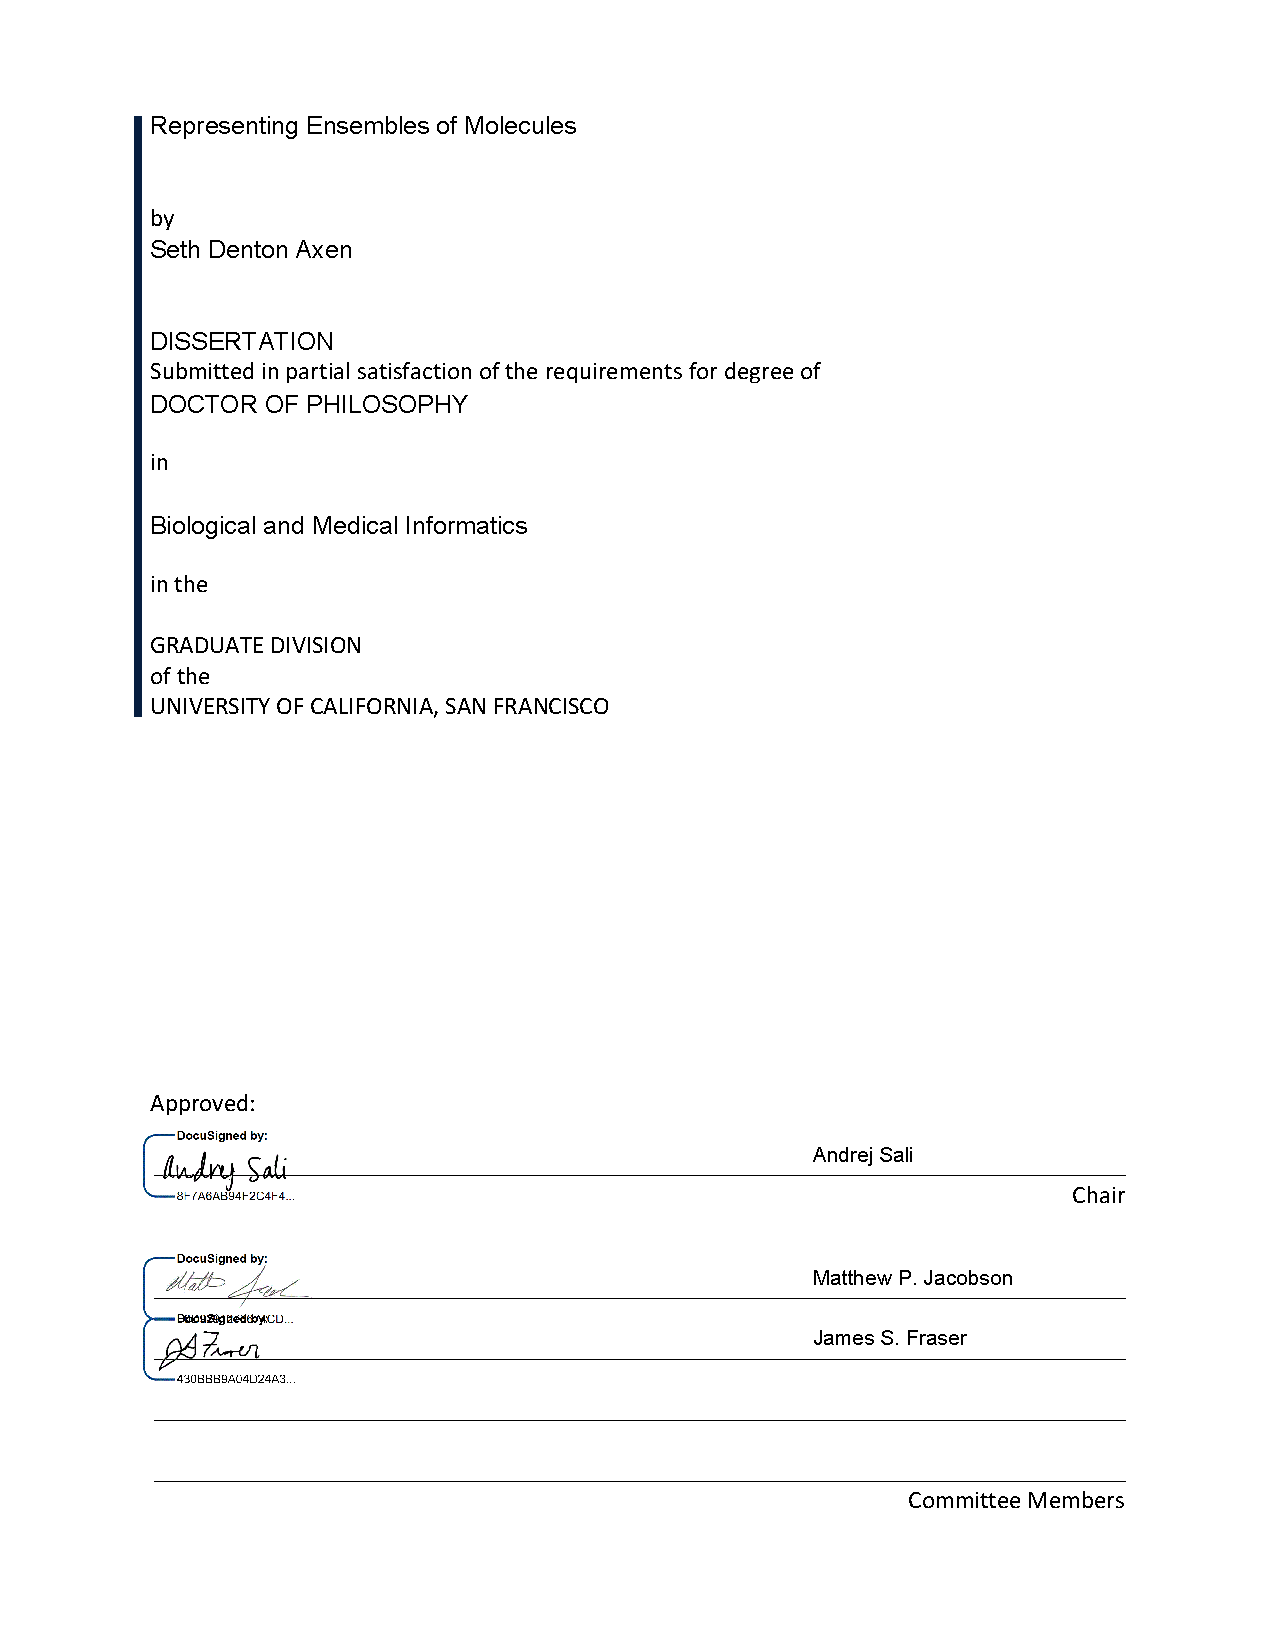
\includepdf[pages=-,width=\paperwidth]{frontmatter/titlepage.pdf}
\begin{center}
	\vspace{1in}  Copyright 2020\par
	\vspace{.1in} by\par
	\makeatletter
	\vspace{.1in} \@author{}
	\makeatother
\end{center}

\doublespacing{}
\chapter*{Acknowledgements}

\begin{centering}
	Greg Nishiyama, for teaching me that science was fun

	Erin Sanders and Cheryl Kerfeld, for taking a chance on me

	Members of the Sali lab, for many thought-provoking debates and good laughs

	Andrej Sali and Mike Keiser, for giving me the freedom to explore

	The administrators and my fellow students in iPQB and CCB, for making UCSF a safe and fun place to learn and wonder

	Ilan Chemmama, for being the best midnight rubber duck

	Joshua Salafsky and Bason Clancy, for inspiration and many fruitful discussions

	The Julia developer community, for the many crucial insights and for making the work so much more enjoyable

	NSF and the ARCS Foundation, who payed the bills so I could have the freedom to think

	Beverly Axen, for teaching me to chase my interests and fight for understanding

	John Axen, for lending me your voice to always keep me going

	My Wolf family, for showing me with your quiet love how to be a better human

	Linda Axen, my partner, my lifeline, my best friend, for your faith in me, for making me better, for so many sacrifices

	August Axen and Anton Axen, for each day making tomorrow look a little brighter

\end{centering}

\chapter*{Contributions}

\section*{\cref{e3fp-paper}}

\fullcite{axenSimpleRepresentationThreeDimensional2017}

% \chapter*{Epigraph}

\begin{center}\textit{to John Axen}\end{center}

\clearpage

\begin{center}
	\makeatletter
	{\Large \textbf{\@title}}

	\@author

	\makeatother

	\vspace{1cm}
	\textbf{Abstract}
\end{center}

Biologically relevant molecules are often dynamic.
That they are not rigid is frequently critical for their function but also makes them immensely challenging to study.
Nevertheless, and perhaps surprisingly, across the fields of cheminformatics and computational biology, algorithms and analyses that ignore the flexibility of such molecules have been widely useful.
To date, most solved protein structures approximate a protein as a single rigid structure, even when data used to determine the structure was clearly derived from many molecules.
Likewise, connectivity or feature fingerprint representations of small molecules have been quite useful for training machine learning methods to predict properties such as whether a molecule might have a high binding affinity to a protein.
Despite the many successes of these approximations, there are many cases where an explicit encoding of the structure and dynamics of a molecule either is required or is reasonably expected to improve the performance of some method.
Such an encoding is called a representation.

As input to a machine learning model for small molecule target prediction, the representation of the molecule encodes the molecule's structure into a format suitable as an input to the machine learning method.
A well-performing representation in this category generally converts the molecule to an array of numbers, encoding as many unique features as possible.
The representation need not be human-interpretable; therefore, it can be a highly compressed view of the input information.

On the other hand, a useful representation for inferring a macromolecular structure has a different set of properties.
Such a representation is a language that defines the world of possible hypothetical structures.
In order to be useful, it must be interpretable; that is, it must be somehow relatable to the actual biological system of interest, and when fitting the structure with data, the representation of the molecule must be accompanied with some representation of the physical process that generated the data.
However, it is easy to make the representation too expressive, making it infeasible to actually explore the representational space for fitting a structure.
Therefore, the currently best available representation for determining a certain structure is usually a compromise based on the nature of the biological question of interest and availability of data and computational resources.
As more detailed biological questions are posed, more information is acquired, and hardware and algorithms become more efficient, more elaborate structural models can be constructed.

There is in general no optimal representation for a molecular structure.
Rather, for each analysis, and even for each stage of an analysis, a different representation may be preferable.
Ideally, the practitioner would have at their disposal a large library of molecular representations designed for different tasks, each with their benefits and limitations well-established.
Furthermore, to be generally useful, these representations should be either easy to implement or have existing efficient, well-tested, stand-alone implementations that can then be integrated into an existing analysis workflow with little additional effort.
This thesis presents two new representations for this library, each for a different class of problems.

\cref{e3fp-paper} presents the Extended Three-Dimensional Fingerprint (E3FP), a simple approach for encoding three-dimensional structural features of small molecules that generalizes widely used methods that use only the molecule's connectivity.
For a given molecule, E3FP generates a bitvector fingerprint that can then be used to train machine learning methods for various tasks.
We showed that the representation in some cases outperformed widely used non-structural representations and even other three-dimensional representations for predicting target-molecule binding pairs.
Moreover, this chapter explored several modifications to E3FP to represent sets of conformers for the same molecule (\ie a molecular ensemble) and showed that these techniques also performed well.

\cref{ensemble-inference,shg-tpf} are adapted from in-preparation manuscripts and introduce a structural representation for Bayesian inference of structural ensembles.
Most techniques for structural inference often either treat a structure as rigid or rely heavily on expensive molecular dynamics techniques to simulate multiple copies of a system, which are perturbed during sampling or post-processing to satisfy data restraints.
This work takes a different approach, approximating the ensemble as a continuous distribution of structures from which measured data can be efficiently simulated through ensemble averaging.
This is achieved by making a number of assumptions about how the structure can be separated into rigid bodies and how those bodies interact.
Techniques from group theory and harmonic analysis on the kinematic groups enable efficient simulation of ensemble averaged data.
The result is the kinematic ensemble representation.
In \cref{ensemble-inference}, the kinematic ensemble representation is applied for ensemble inference using nuclear magnetic resonance (NMR) nuclear Overhauser effect (NOE) measurements, while \cref{shg-tpf} extends the technique for ensemble inference using second-harmonic generation (SHG) and two-photon fluorescence (TPF) measurements.
To keep the main text accessible, the theory and derivations underpinning the kinematic ensemble representation are given in \cref{ensemble-inference-si,shg-tpf-si}, while \cref{ad-rules,ad-power-series} are stand-alone explanations of some of the automatic differentiation methods used in this work.

\tableofcontents
\listoffigures
\listoftables

% CHAPTERS

\clearpage
\pagestyle{fancy} % header
\pagenumbering{arabic}
\setcounter{page}{1}

\subfile{chapters/chapter01/chapter01}
\subfile{chapters/chapter02/chapter02}
\addtocontents{toc}{\protect\newpage} % avoid dangling at end of page
\subfile{chapters/chapter03/chapter03}

% APPENDIX

\appendix
\subfile{chapters/appendixa/appendixa}
\subfile{chapters/appendixb/appendixb}
\subfile{chapters/appendixc/appendixc}
\subfile{chapters/appendixd/appendixd}

% \printglossary[title=List of Terms]

% \listoftodos


\includepdf[pages=-,width=\paperwidth]{backmatter/publishing_agreement.pdf}

\end{document}
